\documentclass[a4paper, 12pt]{article}%тип документа

%отступы
\usepackage[left=2cm,right=2cm,top=2cm,bottom=3cm,bindingoffset=0cm]{geometry}

%Русский язык
\usepackage[T2A]{fontenc} %кодировка
\usepackage[utf8]{inputenc} %кодировка исходного кода
\usepackage[english,russian]{babel} %локализация и переносы

%Вставка картинок
\usepackage{wrapfig}
\usepackage{graphicx}
\graphicspath{{pictures/}}
\DeclareGraphicsExtensions{.pdf,.png,.jpg}

%Графики
\usepackage{multirow}
\usepackage{pgfplots}
\pgfplotsset{compat=1.9}

%Математика
\usepackage{amsmath, amsfonts, amssymb, amsthm, mathtools}

%Заголовок
\author{Валеев Рауф Раушанович \\
группа 825}
\title{\textbf{Работа 2.4.1 \\ 
Определение теплоты испарения жидкости}}
\begin{document}
\maketitle
\section*{Цель работы}
\begin{enumerate}
\item Измерение давления насыщенного пара жидкости при разной температуре
\item Вычисление по полученным данным теплоты испарения с помощью уравнения Клапейрона-Клаузиуса.
\end{enumerate}
\section*{Теоретическая справка}
\subsection*{Уравнение Клапейрона-Клаузиуса}
Запишем уравнение для свободной энергии Гиббса и дифференциал из 1 и 2 начал термодинамики
\[G = U + PV - TS\]
\[dG = -SdT + VdP\]
Отсюда следует, что если в термодинамической системе не изменяется давление и температура, то потенциал Гиббса так же остается неизменным.

Пусть система состоит из фаз 1 и 2, массы которых равны $m_1$ и $m_2$ соответственно. Удельные термодинамические потенциалы обозначим $\gamma_1 (P, T)$ и $\gamma_2 (P, T)$. Тогда 
\[G = \gamma_1 (P, T) m_1 + \gamma_2 (P, T) m2\]
При фазовом переходе давление и температура не меняются, поэтому не меняется и $G$, и $\gamma_1 (P, T)$, и $\gamma_2 (P, T)$ из условия равновесия. Меняются лишь массы. При этом общая масса всей системы не меняется. Из всего вышеперечсисленного следует, что
\[dm_1 + dm_2 = 0\]
\[dG = 0 = \gamma_1 dm_1 + \gamma_2 dm_2\]
\[\gamma_1 (P, T) = \gamma_1 (P, T)\]
Отсюда получается, что условие равновесия фаз эквивалентно условию равновесия их удельных потенциалов Гиббса. Отсюда получаем
\[d \gamma_1 (P, T) =  -s_1 dT + v_1 dP = d \gamma_2 (P, T) = -s_2 dT + v_1 dP\]
\[d \gamma_1 = d \gamma_2 \Rightarrow\]
\[\dfrac{dP}{dT} = \dfrac{s_2 - s_1}{v_2 - v_1}\]
при $T = const$ имеем, что
\[s_2 - s_1 = \dfrac{q}{T}\]
\[\dfrac{dP}{dT} = \dfrac{q}{T(v_2 - v_1)}\]
Поскольку в данной работе температура далека от критической, то газ можно считать идеальным и можно пренебреч $v_1$ по сравнению с $v_2$, то есть 
\[v_2 = \dfrac{RT}{P}\]
\[q = \dfrac{RT^2}{ P} \dfrac{dP}{dT} = -R \dfrac{d(\ln P)}{d(1/T)}\]
\subsection*{Экспериментальная установка}
\begin{figure}[h]
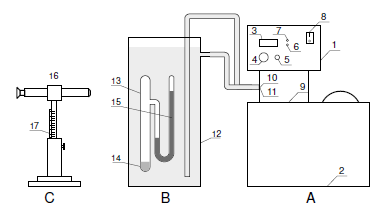
\includegraphics[width = 0.9\textwidth]{1.png}
\caption{Схема установки}
\end{figure}
Здесь блок А - нагревательный элемент, блок В - исследуемый сосуд и С - измерительный микроскоп.
\section*{Ход работы}
\begin{enumerate}
\item Измеряем высоту столба ртути в монометрах при повышении температуры, затем находим разность и по ним считаем разность давлений.
\newpage
\item Проводим те же измерения при понижении температуры. Все данные записываем в таблицу.
\begin{table}[h]
\center{
\begin{tabular}{|c|c|c|c|c|c|c|c|}
\hline
$T, K$ & $\sigma _T, K$ & $h_1, cm$ & $h_2, cm$ & $\Delta h, cm$ & $\sigma _h, cm$ & $p$, Па & $\sigma_p$, Па \\ \hline
294,0 & 0,1 & 4,4 & 8,4 & 4,0 & 0,1 & 5300 & 100 \\ \hline
295,0 & 0,1 & 4,3 & 8,5 & 4,2 & 0,1 & 5600 & 100 \\ \hline
296,4 & 0,1 & 4,2 & 8,6 & 4,4 & 0,1 & 5800 & 100 \\ \hline
297,0 & 0,1 & 4,1 & 8,7 & 4,6 & 0,1 & 6100 & 100 \\ \hline
298,0 & 0,1 & 4,0 & 8,8 & 4,8 & 0,1 & 6300 & 100 \\ \hline
299,0 & 0,1 & 3,8 & 9,0 & 5,2 & 0,1 & 6900 & 100 \\ \hline
300,0 & 0,1 & 3,6 & 9,2 & 5,6 & 0,1 & 7400 & 100 \\ \hline
301,0 & 0,1 & 3,5 & 9,3 & 5,8 & 0,1 & 7700 & 100 \\ \hline
302,0 & 0,1 & 3,3 & 9,5 & 6,2 & 0,1 & 8200 & 100 \\ \hline
303,0 & 0,1 & 3,1 & 9,7 & 6,6 & 0,1 & 8700 & 100 \\ \hline
304,0 & 0,1 & 2,9 & 9,9 & 7,0 & 0,1 & 9300 & 100 \\ \hline
305,0 & 0,1 & 2,7 & 10,1 & 7,4 & 0,1 & 9800 & 100 \\ \hline
306,0 & 0,1 & 2,4 & 10,4 & 8,0 & 0,1 & 10600 & 100 \\ \hline
307,0 & 0,1 & 2,2 & 10,6 & 8,4 & 0,1 & 11100 & 100 \\ \hline
308,0 & 0,1 & 2,0 & 10,8 & 8,8 & 0,1 & 11600 & 100 \\ \hline
309,0 & 0,1 & 1,7 & 11,1 & 9,4 & 0,1 & 12500 & 100 \\ \hline
310,0 & 0,1 & 1,4 & 11,4 & 10,0 & 0,1 & 13200 & 100 \\ \hline
\end{tabular}
}
\caption{$P$ от $T$ при нагреве}
\end{table}

\begin{table}[h]
\center{
\begin{tabular}{|c|c|c|c|c|c|c|c|}
\hline
$T, K$ & $\sigma _T, K$ & $h_1, cm$ & $h_2, cm$ & $\Delta h, cm$ & $\sigma _h, cm$ & $p$, Па & $\sigma_p$, Па \\ \hline
308,4 & 0,1 & 1,9 & 10,9 & 9,0 & 0,1 & 11900 & 100 \\ \hline
307,0 & 0,1 & 2,2 & 10,6 & 8,4 & 0,1 & 11100 & 100 \\ \hline
305,4 & 0,1 & 2,6 & 10,2 & 7,6 & 0,1 & 10100 & 100 \\ \hline
304,4 & 0,1 & 2,8 & 10,0 & 7,2 & 0,1 & 9500 & 100  \\ \hline
302,4 & 0,1 & 3,2 & 9,6 & 6,4 & 0,1 & 8500 & 100 \\ \hline
300,8 & 0,1 & 3,5 & 9,3 & 5,8 & 0,1 & 7700 & 100 \\ \hline
299,4 & 0,1 & 3,7 & 9,1 & 5,4 & 0,1 & 7100 & 100 \\ \hline
297,0 & 0,1 & 4,1 & 8,7 & 4,6 & 0,1 & 6100 & 100 \\ \hline
\end{tabular}
}
\caption{$P$ от $T$ при охлаждении}
\end{table}
\newpage
\item Строим график в координатах $1/T$ и $\ln P$.
\begin{figure}[h]
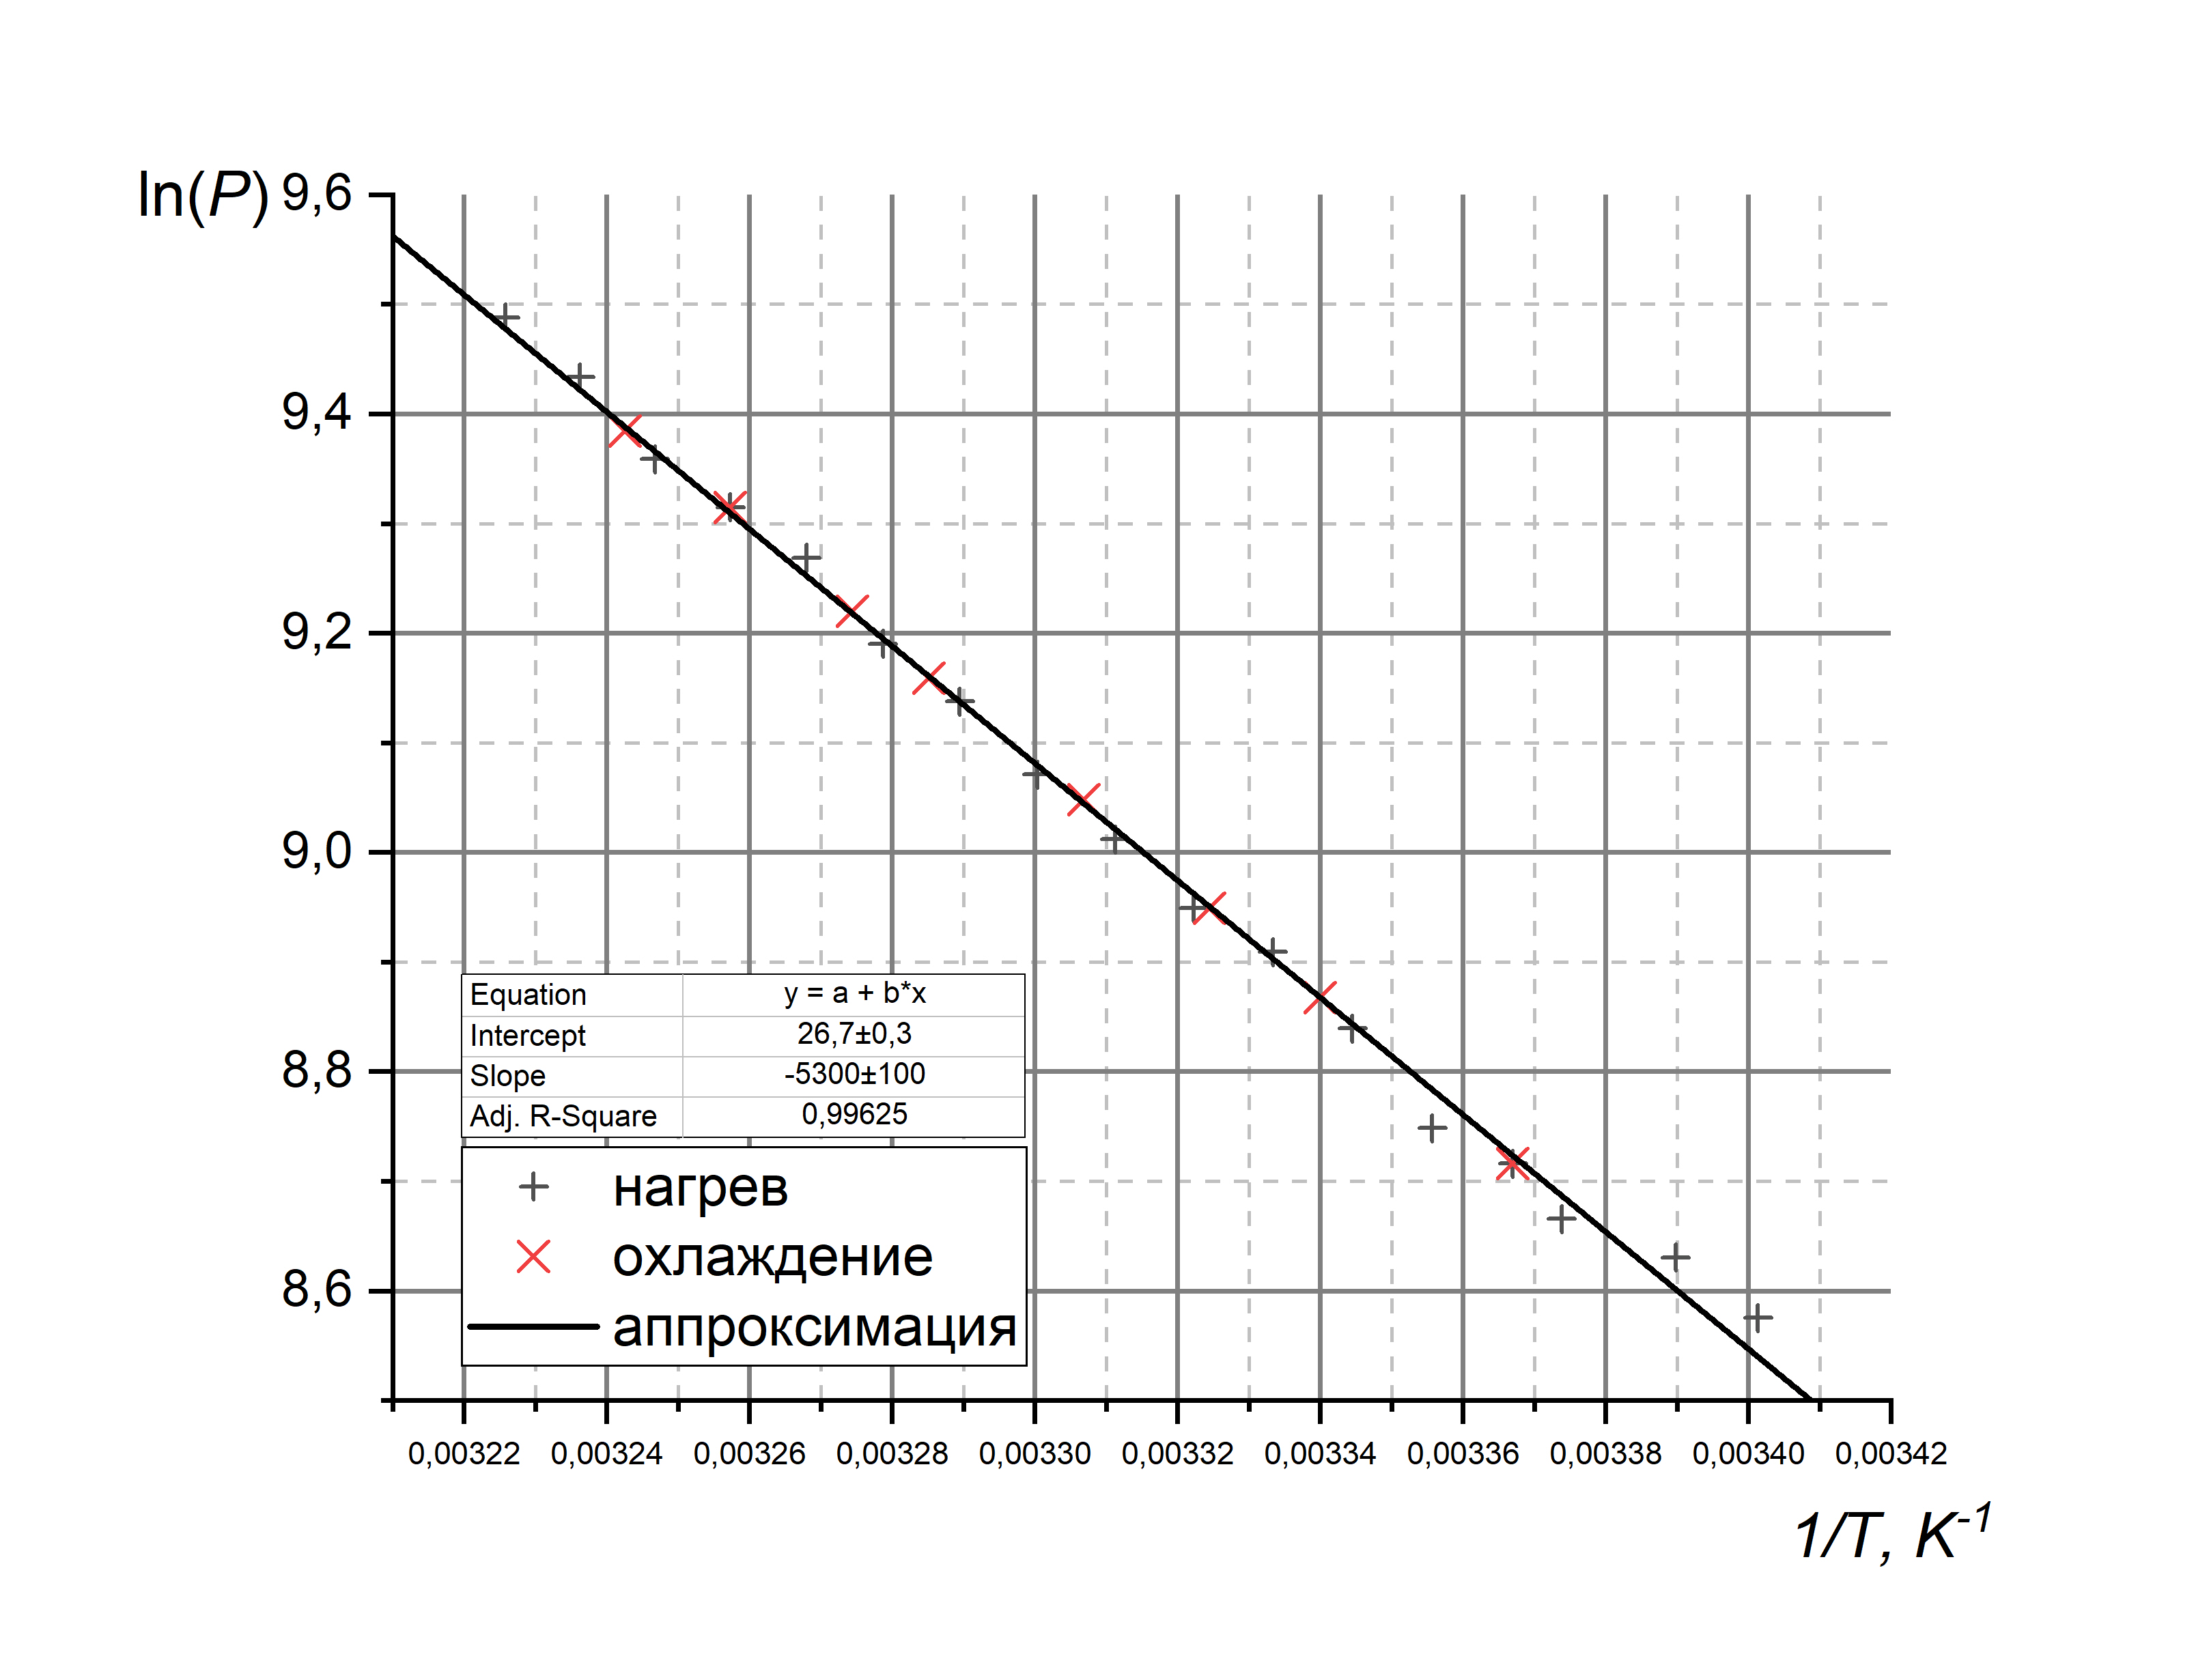
\includegraphics[width = \textwidth]{2.jpg}
\caption{График зависимости $\ln P$ от $1/T$}
\end{figure} 
\item Вычисляем $L$ по первому графику.
\begin{table}[h]
\begin{tabular}{|c|c|c|c|c|c|}
\hline
$\dfrac{d(\ln P)}{d(1/T)}, K$ & $\sigma_{d(\ln P)/d(1/T)}, K$ & $L$, Дж/моль & $\sigma_L$, Дж/моль & $L$, Дж/г & $\sigma_L$, Дж/г \\ \hline
-5300 & 100 & 44000 & 1000 & 960 & 20 \\ \hline
\end{tabular}
\caption{Результаты полученные из первого графика}
\end{table} 
\newpage
\item Строим график в координатах $T$ и $P$.
\begin{figure}[h]
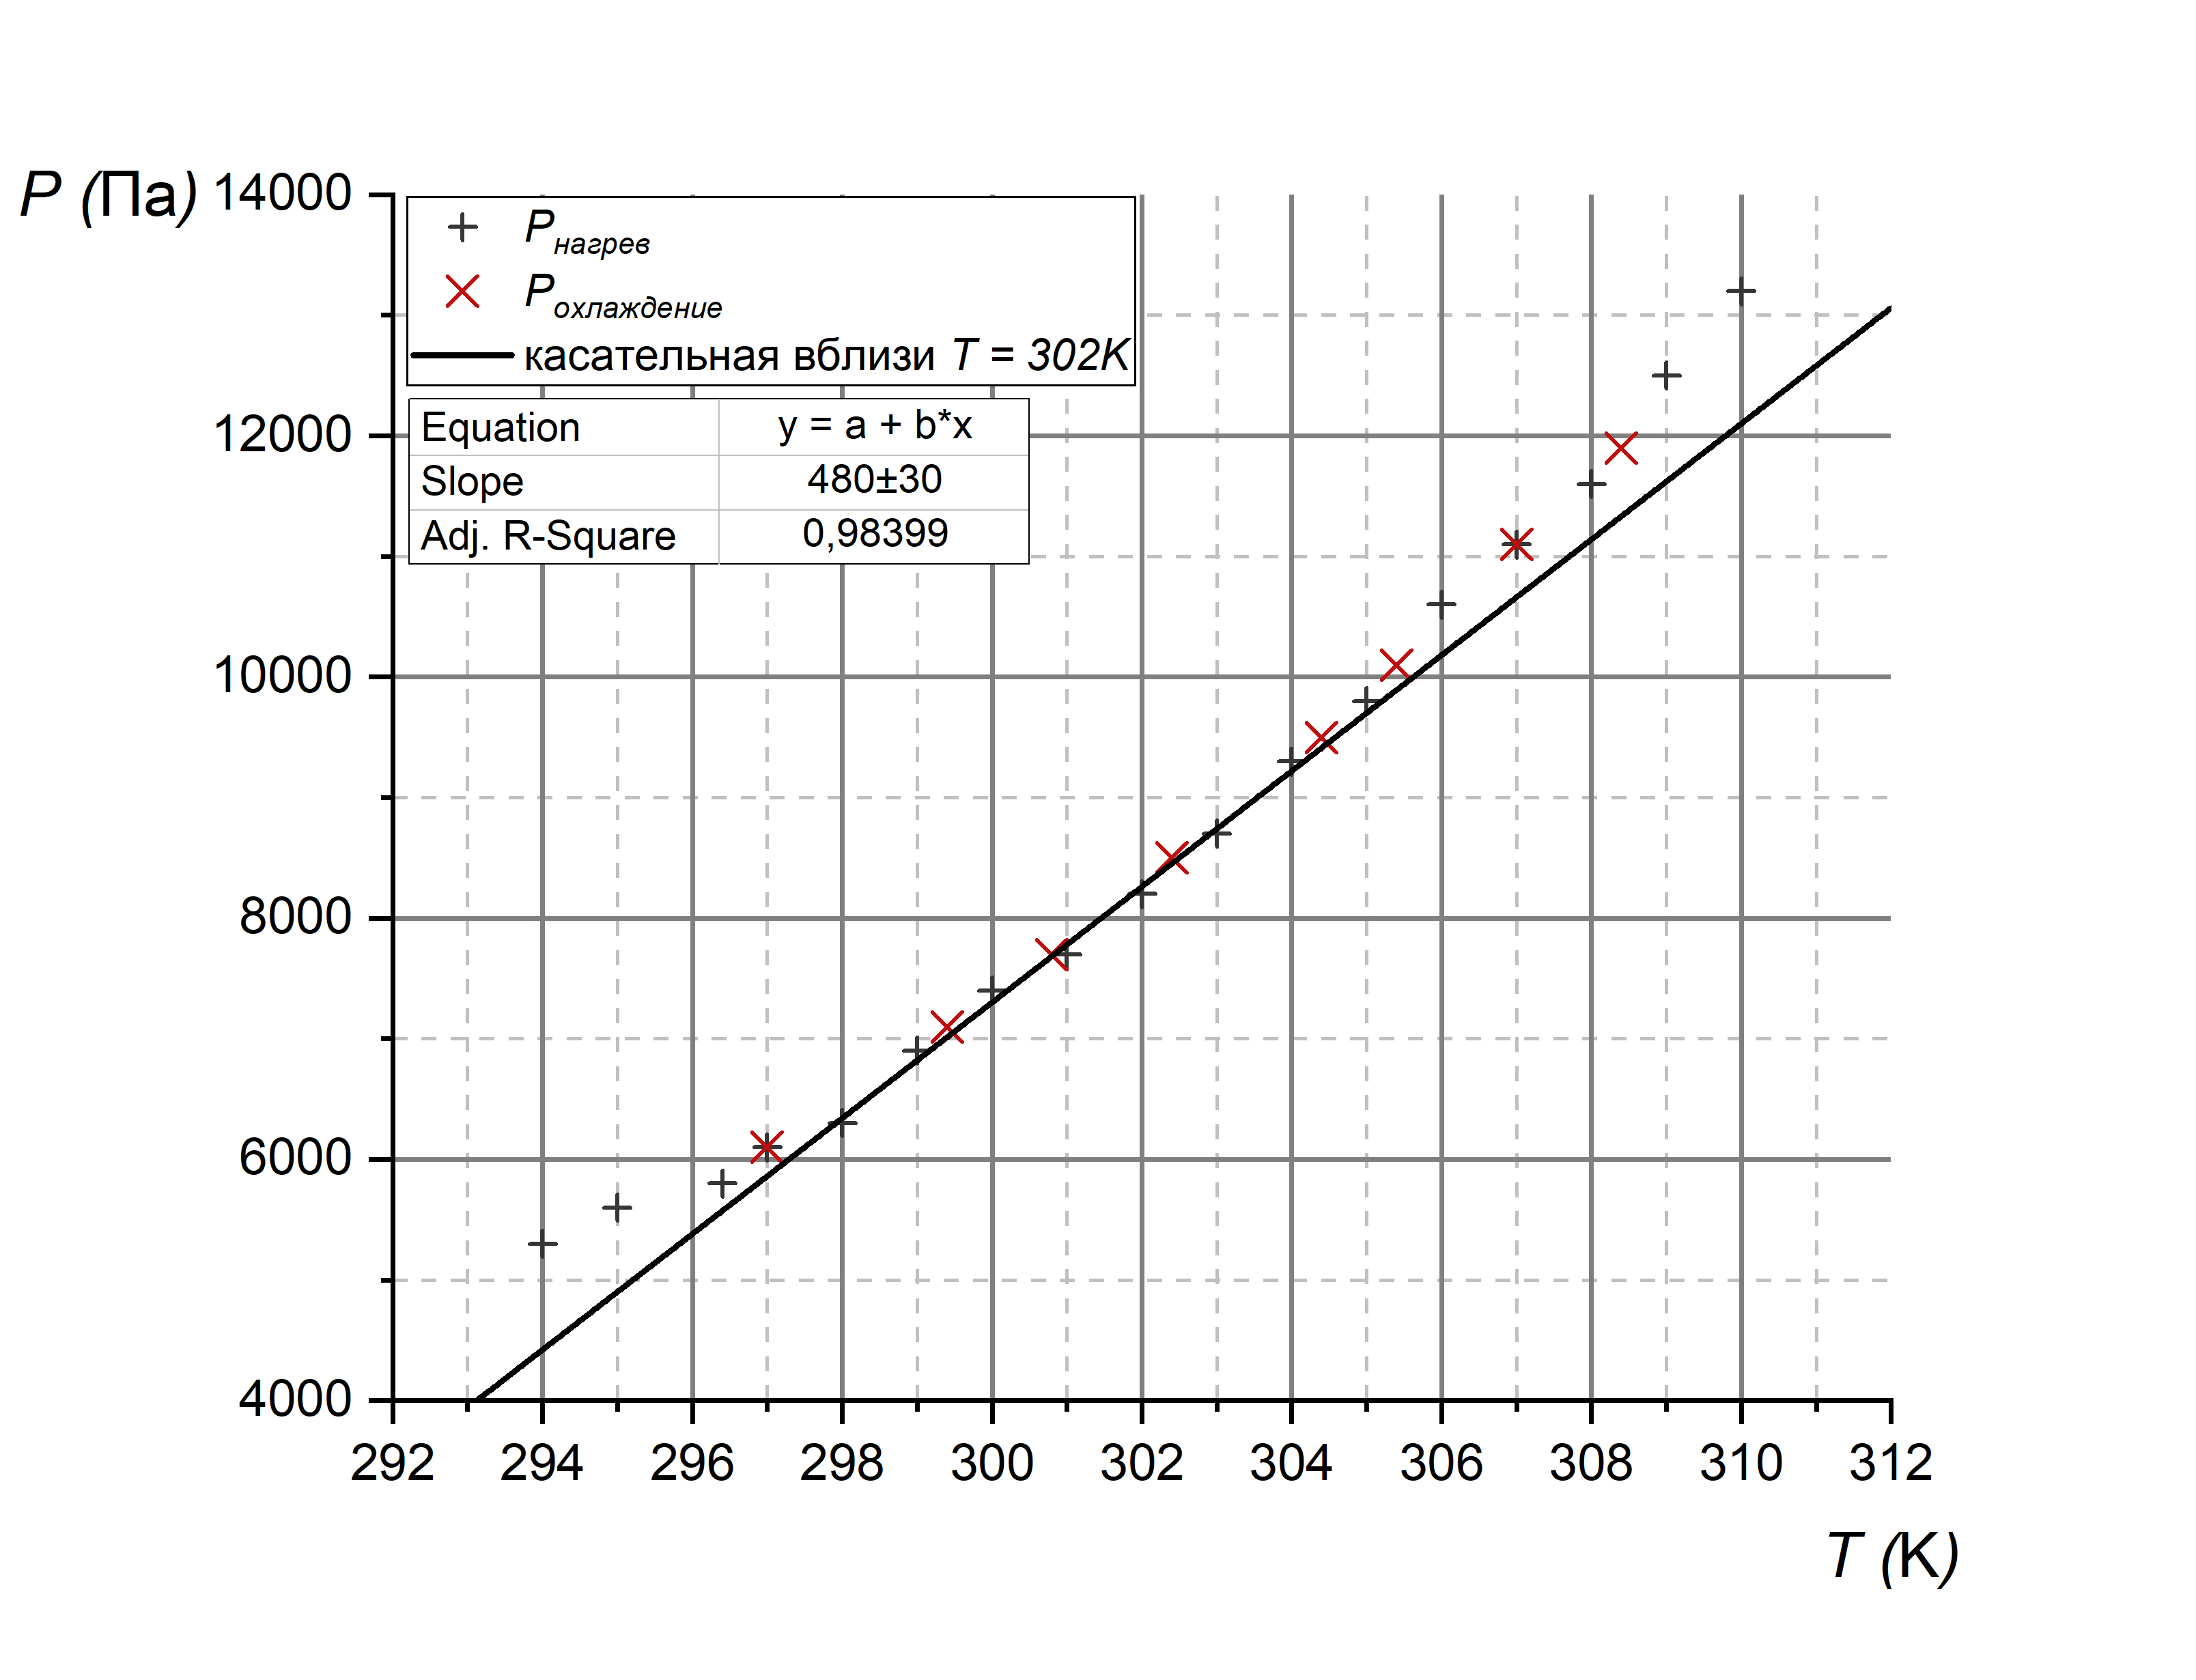
\includegraphics[width = \textwidth]{3.jpg}
\caption{График зависимости $P$ от $T$}
\end{figure} 
\item Вычислим $L$ по второму графику, например вблизи точки $T = 302K$. Для этого построим касательную в данной точке, найдем $v_2$ по формуле $v_2 = \dfrac{RT}{\mu P}$ и далее из формулы 
\[\dfrac{dP}{dT} = \dfrac{L}{T(v_2 - v_1)}\]
Принебрегая $v_1$ по сравнению с $v_2$ мы получим 
\[L \approx \dfrac{dP}{dT} \cdot T \cdot v_2\]
\begin{table}[h]
\begin{tabular}{|c|c|c|c|c|}
\hline
$dfrac{dP}{dT},\text{Па}/K$ & $\sigma_{dP/dT},  \text{Па}/K$ & $v_2, m^3/ \text{моль}$ & $L$, Дж/г & $\sigma_L$, Дж/г \\ \hline
480 & 30 & 2000 & 960 & 60 \\ \hline
\end{tabular}
\caption{Результаты для второго графика}
\end{table}
\item Сравнивая полученные результаты можно сделать вывод, что нахождение по первому графику более точное, нежели по второму. Исходя из таблицы мы видим, что наши результаты довольно точно совпадают с табличными, то есть с $L = 920 \text{Дж}/\text{г}$ при $T = 302 K$
\end{enumerate}
\end{document}